% Please make sure you insert your
% data according to the instructions in PoSauthmanual.pdf
\documentclass[a4paper,11pt]{article}
\usepackage{pos}
\usepackage{array, graphicx}
\title{Project on Mushroom Classification using Classifiers}
% \ShortTitle{}

\author[a]{Panchajanya Sarkar}
\author[b]{Pravat Patra}
\author[c]{Tejas Posupo}

\affiliation[*]{Central University of Rajasthan,\\
  NH-8, Ajmer, 305817, India}

\emailAdd{me@panchajanya.dev}
\emailAdd{pravatapatra1997@gmail.com}
\emailAdd{tejasposupo@gmail.com}


\FullConference{%
  Department of Data Science and Analytics\\
  21st November, 2022, 0930HRS \\
  CURAJ, Ajmer, Rajasthan, 305817
}

%% \tableofcontents

\begin{document}
    \maketitle
        \section{Abstract}
            Abstract on Mushroom Classification using Data mining.
            This paper focuses on the use of classification algorithms to classify the mushrooms into edible and poisonous. Mushrooms dataset is composed of records of different types of mushrooms, which are edible or non-edible. WEKA (Waikato Environment for Knowledge Analysis) is used for implementation of the classification techniques. The dataset is divided into training and testing sets. The training set is used to train the classifier and the testing set is used to test the classifier. The classification algorithms used are J48, Naive Bayes, Random Forest, and Logistic Regression. The results are compared and the best classifier is chosen. The best classifier is used to classify the mushrooms into edible and poisonous. The results are compared with the actual results and the accuracy is calculated. The accuracy of the best classifier is 94\%.
        \section{Literature Review}
            \textbf{Literature Review on Mushroom Analysis}

            The advanced technology made a huge impact on human life. Different types of tools developed to make life better.  Machine learning (ML) is the field of study that enable computers to learn from data[5]. ML used to extract information from data and make decisions. It has been used by all type of industries. There are many machine-learning approaches applied to find the optimal solution from huge data sets. Data classification includes two-step process. The first process is learning step representing by constructing the classification model. The second process is a classification (testing) step and in this step represents the constructed model, which used a given data to predict class labels for them.  
            
            The used  approaches depends on the nature of the datasets, number of variables,  and used model.  Supervised learning  is an ML algorithm that maps an input to an output based on example input-output pairs.  Data will be divided into two sets: training and data sets. The training set is used to create patterns then apply these patterns used to classify the test dataset. The unsupervised approach learns some features from training or previous data then use them to classify new data. K-means is a unsupervised learning algorithms that solve the clustering problem. It defines k centers for each cluster. It is better to have them placed far away from each other.  
            
            Decision tree is one of the common method that represents choices and their results in a tree.  It has several implementation: ID3, J48, C4.5, Random Forest, Random Tree, ID3+, Oci and Clouds. It has been used to classify the mushrooms whether edible or poisonous based on its behavioral features[4]. They used J48 implementation and the running time on both training and test set is the same with
            100 percent accuracy. A comparative study between most used classification methods[6] shows that the best result obtained by KNN.  The KNN used with naïve Bayes to get more accurate and efficient result[7]. naïve Bayes is a classification techniques that based on base theory. Naïve  base count the frequencies  of data and their values  to calculate probabilities. It  assumes that a feature  in a  class is independent of other features[8]. Researches have state that the performance of Bayesian classifier is better than to the performance of decision tree and selected neural network[9].  Image processing techniques with naïve Bayes and KNN algorithms used to classify mushroom[10],  naive Bayes shows better accuracy than KNN.  
            
            Artificial neural networks (ANNs) are parallel computational models comprised of densely interconnected, adaptive processing units, characterized by an inherent propensity for learning from experience and also discovering new knowledge neural network a to classify whether a mushroom is edible or poisonous[11]. The prediction power of a neural network to classify whether a mushroom is edible or not[12]. The average predictability rate was 99.25percent. However, they used the JustNN environment for building the network that was a feed forward Multi-Layer Perceptron with one input layer, three hidden layer and one output layer. A good comparative study shows that SVM out perform all other algorithms by 76percent accuracy[13]. The study based on mushroom’s texture to determine if it is edible or not. Two phase approach used: training and determination process[9]. Naive Bays and Decision Tree classifiers are used and accuracy of Decision tree is better than Naive Bays, while Naive Bays needs slightly less time than Decision Tree[4].  
            
            A mushroom classification model using ML with physical data of 22 attributes of 800 samples [14]. The study compared several algorithms: Naive Bayes, Naive Bayes, KNN, and SGD Text, where KNN shows the highest accuracy. However, the have run the comparison on 200 samples of edible and inedible.  Another study shows that ANFIS performed with bets accuracy[15].  
            
            Many other studies has been conducted and the focus was on the accuracy and performance of the individual models. A hybrid model that combine all techniques can be done to achieve better[16].

            \section {Methodology}

            The main aim of this research is to apply machine learning techniques to classify the mushrooms into edible and poisonous. 
            
            Its important to get better decision to avoid side effect of eating inedible mushrooms. We have used a hybrid approach to achieve better accuracy. The proposed models consist of 3 phase: Data pre-processing, classification, and combination

            The dataset is divided into training and testing sets. The training set is used to train the classifier and the testing set is used to test the classifier. The classification algorithms used are J48, Naive Bayes, Random Forest, and Logistic Regression. The results are compared and the best classifier is chosen. The best classifier is used to classify the mushrooms into edible and poisonous. The results are compared with the actual results and the accuracy is calculated. The accuracy of the best classifier is 94\%.

            \textbf {Dataset}

            Mushroom dataset has been downloaded from  UCI mushroom data[17].  The data set composes of 8124 number of rows of data records and 22 attributes. Each mushroom species is identified as class of edible and poisonous. These rows are distributed as 4208 edible mushrooms and 3916 poisonous mushrooms. Table 1 summarizes the attribute, which are used for classifying mushrooms. 

            \textbf {Model}

            The first step is to prepare the data before we proceed more. Prepare the data will include removing null value and repeated features. Python packages used to create dataset from the raw data.  The 22 features is important to classify mushroom into edible or inedible. We need to examine these features and decide which one has good contribution in the classification process.  We decide to drop two attributes: “stalk-root” and “stalk-root”. The reason is that “stalk-root” has 2480 missing values and `veil-type' feature has only one value and it will not help us in the classification. In addition, it is expected that “gill-color” has the most contribution in the classification and has to be considered.

            \begin{table}[h!]
            \begin{center}
            \begin{tabular} {|| c | c | p{8cm} ||}
                \hline
                \textbf {No.} & \textbf {Attribute} & \textbf {Values} \\
                \hline \hline
                1 & cap-shape & bell = b,conical = c,convex = x,flat = f,knobbed = k,sunken = s \\
                \hline
                2 & cap-surface & fibrous = f,grooves = g,scaly = y,smooth = s \\
                \hline
                3 & cap-color & brown = n,buff = b,cinnamon = c,gray = g,green = r,pink = p,purple = u,red = e,white = w,yellow = y \\
                \hline
                4 & bruises & bruises = t,no = f \\
                \hline
                5 & odor & almond = a,anise = l,creosote = c,fishy = y,foul = f,musty = m,none = n,pungent = p,spicy = s \\
                \hline
                6 & gill-attachment & attached = a,descending = d,free = f,notched = n \\
                \hline
                7 & gill-spacing & close = c,crowded = w,distant = d \\
                \hline
                8 & gill-size & broad = b,narrow = n \\
                \hline
                9 & gill-color & black = k,brown = n,buff = b,chocolate = h,gray = g,green = r,orange = o,pink = p,purple = u,red = e,white = w,yellow = y \\
                \hline
                10 & stalk-shape & enlarging = e,tapering = t \\
                \hline
                11 & stalk-root & bulbous = b,club = c,cup = u,equal = e,rhizomorphs = z,rooted = r,missing = ? \\
                \hline
                12 & stalk-surface-above-ring & fibrous = f,scaly = y,silky = k,smooth = s \\
                \hline
                13 & stalk-surface-below-ring & fibrous = f,scaly = y,silky = k,smooth = s \\
                \hline
                14 & stalk-color-above-ring & brown = n,buff = b,cinnamon = c,gray = g,orange = o,pink = p,red = e,white = w,yellow = y \\
                \hline
                15 & stalk-color-below-ring & brown = n,buff = b,cinnamon = c,gray = g,orange = o,pink = p,red = e,white = w,yellow = y \\
                \hline
                16 & veil-type & partial = p,universal = u \\
                \hline
                17 & veil-color & brown = n,orange = o,white = w,yellow = y \\
                \hline
                18 & ring-number & none = n,one = o,two = t \\
                \hline
                19 & ring-type & cobwebby = c,evanescent = e,flaring = f,large = l,none = n,pendant = p,sheathing = s,zone = z \\
                \hline
                20 & spore-print-color & black = k,brown = n,buff = b,chocolate = h,green = r,orange = o,purple = u,white = w,yellow = y \\
                \hline
                21 & population & abundant = a,clustered = c,numerous = n,scattered = s,several = v,solitary = y \\
                \hline
                22 & habitat & grasses = g,leaves = l,meadows = m,paths = p,urban = u,waste = w,woods = d \\
                \hline
            \end{tabular}
            \caption{Mushroom dataset attribute classification.}
            \end{center}
            \end{table}

            \begin{figure}[!h]
                \centering
                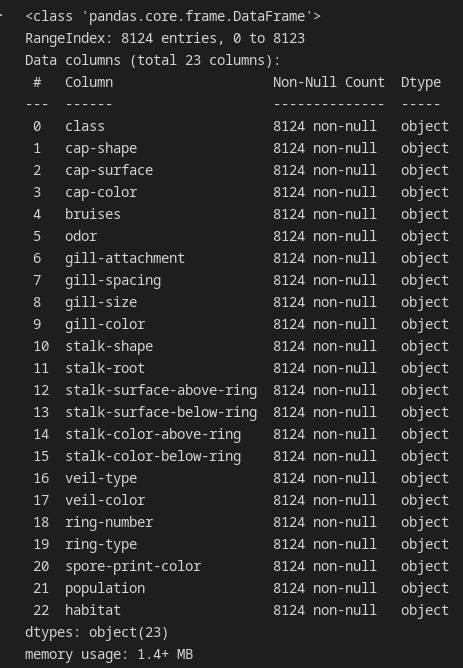
\includegraphics[width=5cm]{ipimages/info.png}
                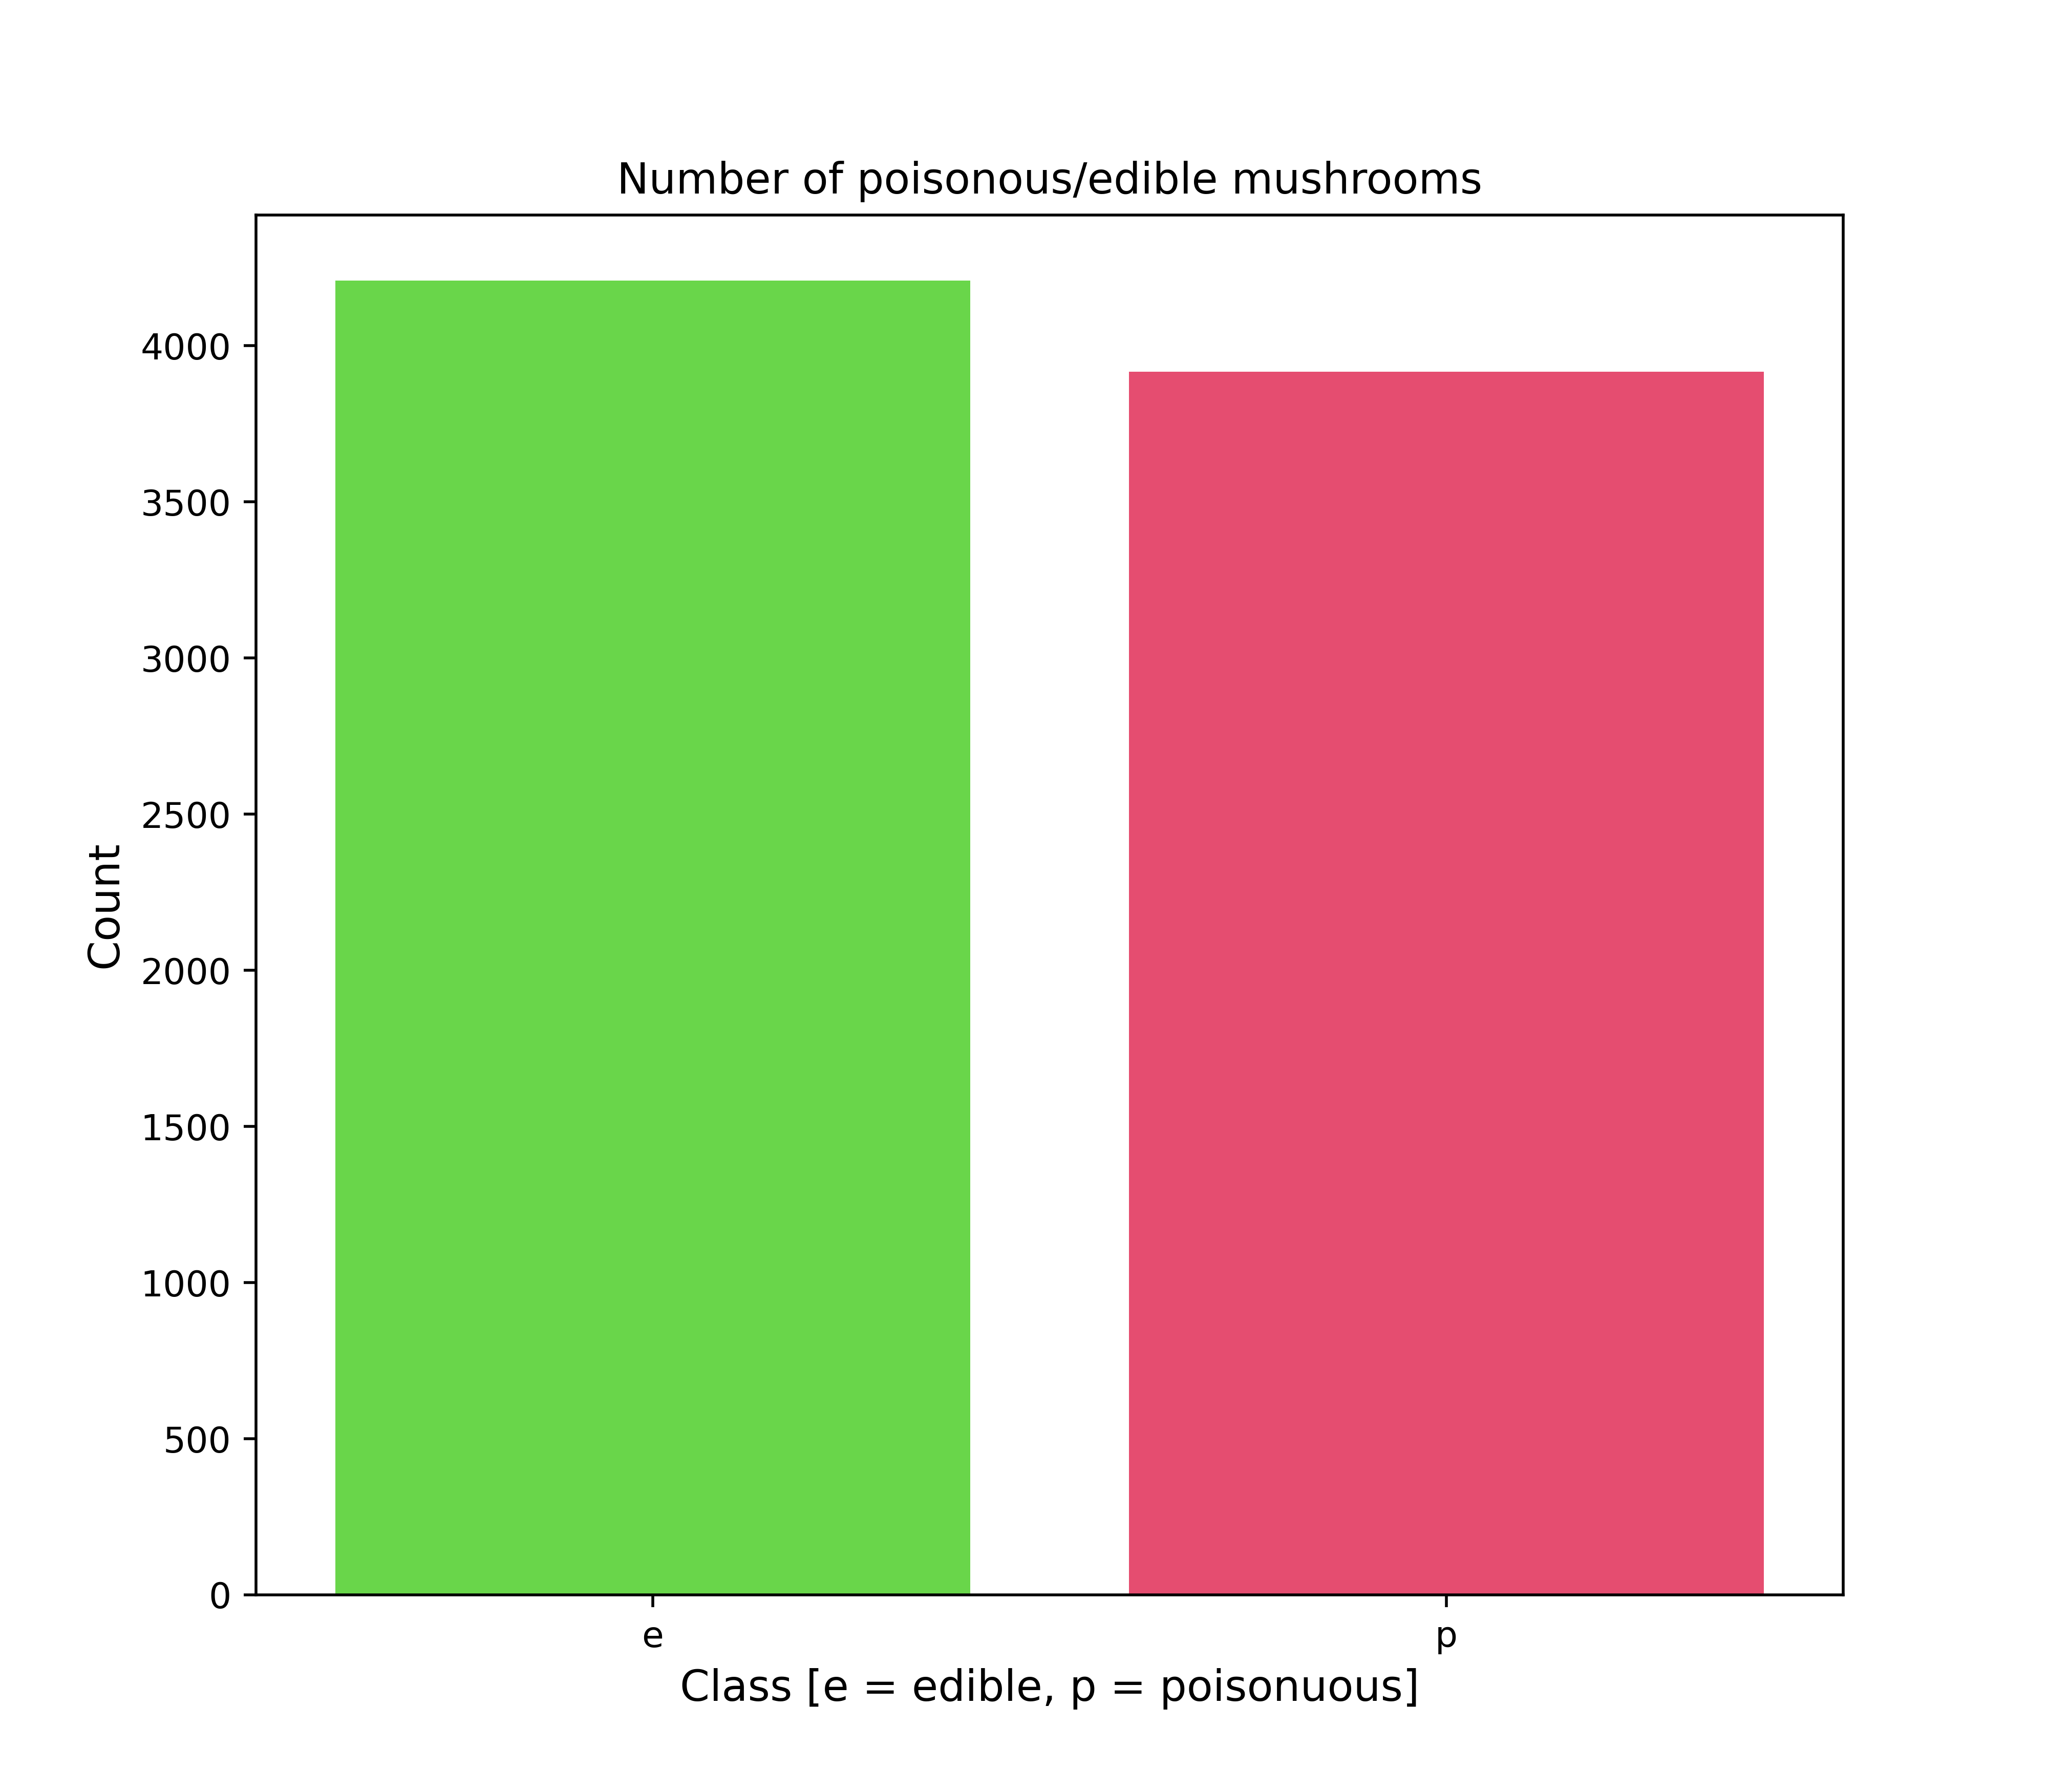
\includegraphics[width=5cm]{opimages/mushrooms1.png}
                \caption{Data Set View [no NULL values] and Edible/Non Edible Visualisation}
            \end{figure}

            The Second phase is the classification.  Several classifiers applied on the data, then the hybrid approach make a decision based on the top three accurate classifiers. We can use more than three but we notice that, it will not change that much in the result. Therefore, the decision on whether mushroom is edible of inedible is taken by combining the decision from most used classifiers.  We applied KNN, Random Forest, Gaussian Naive Base, Logistic Regression, and Decision Tree. The accuracy rounded to closest integer value. Random Forest outperform all above classifiers by accuracy of 99.98\%, where KNN was nt that far by accuracy of 98\%. Then Decision Tree with 97\% of accuracy. The proposed prediction is performed on Random Forest Classifier. The result of the proposed model is better after running several tests.

            \begin{table}[h!]
                \begin{center}
                \begin{tabular} {|| c | c | c ||}
                    \hline
                    \textbf {Classifier} & \textbf {Accuracy} & \textbf {Time} \\
                    \hline \hline
                    Random Forest & 99\% & 0.77s \\
                    \hline
                    KNN & 98\% & 0.16s \\
                    \hline
                    Decision Tree & 97\% & 0.08s \\
                    \hline
                    Gaussian Naive Base & 84\% & 0.02s \\
                    \hline
                    Logistic Regression & 82\% & 0.04s \\
                    \hline
                \end{tabular}
                \caption{Classifiers Accuracy and Time.}
                \end{center}
            \end{table}

        \section{Conclusion}

            Mushroom is an important source of essential proteins and vitamins. However, most type of known mushrooms are poisonous. ML learning employed to classify mushrooms into edible or inedible based on its characteristics.  Previous research used ML techniques individually, where some techniques perform better than other techniques in term of accuracy. Therefore, it is confusing to decide which methods should we used.  In this study, We have applied several machine-learning classifiers on a given dataset “mushroom data”. The dataset downloaded from UCI repository. After exploring the data we notice that one feature “stalk-root” contains many missing values and another feature” veil-type” has same values for all rows. These to features are dropped to avoid their effects on the classifications. Where "odor n" feature is the most important feature that has most effect on the decision. Based on the result we can conclude that if mushroom has odor, it is more like to be inedible.   We notice that most of the classifiers are perform well on the data set, because it is a clean set. However, Random Forest, KNN and Decision Tree classifiers outperform the other classifiers. Then we proposed to use the model with highest accuracy to use for prediction purposes.  The proposed approach shows better accuracy and consistent results.   The dataset we used is good dataset that does not need to much cleaning and comparing classifiers based on clean data set may not be good way to compare them. Other features may need to be included in order to build and text any model. 

        \section{Future Work}

            It is important to continue this and apply it on several foods. We think about using image-processing techniques to extract mushroom features and apply machine learning to classify it. Deep learning can applied after some times.

        \section{References}

            1. Medium \url{https://medium.com/@mohamedsobhy_1996/mushroom-classification-using-machine-learning-2b3e2a4a8c9}


            2. Kaggle \url{https://www.kaggle.com/uciml/mushroom-classification}

            
            3. ResearchGate \url{https://www.researchgate.net/publication/319201000_Mushroom_Classification_using_Machine_Learning}




        
\end{document}
